\section{Kết quả}
\label{sec:results}

% ---------------------------------------------------------------------------
\subsection{RQ1: khi nào DLinear và NLinear thu về Linear}
\label{sec:rq1}

\paragraph{Ba dự đoán.} Từ biểu diễn $\Weff$ ở \secref{sec:method-models}, Phụ lục~\ref{app:derivation} suy ra ba dự đoán:
\begin{enumerate}[label=(\arabic*)]
    \item Khi $\lambda = 0$, DLinear trùng Linear: $[P, I - P]$ có hạng $L$ nên tập các $\Weff$ của DLinear đúng bằng tập của Linear.
    \item Khi $\lambda > 0$, DLinear tách khỏi Linear: weight decay của DLinear là ridge trong metric $N^{-1}$ thay vì ridge đẳng hướng, nên mức tách phụ thuộc kernel $k$.
    \item NLinear tách khỏi Linear ở mọi $\lambda$, vì nó là Linear với ràng buộc tổng hàng bằng $1$.
\end{enumerate}

\tabref{tab:b2} tóm tắt phép kiểm trên ETTh1, $H = 96$. Nghiệm tối ưu được giải trong chính tham số hóa của module DLinear, NLinear của repo LTSF-Linear, rồi nạp vào module. Gradient qua autograd tại nghiệm gần bằng $0$ so với lúc khởi tạo, nên nghiệm là cực tiểu toàn cục của hàm lồi. Cả ba dự đoán đều đúng.

\begin{center}
\small
% Tự động sinh bởi scripts/report/make_tables.py từ results/. KHÔNG SỬA TAY.
\begin{tabular}{@{}p{0.2\linewidth}p{0.36\linewidth}p{0.36\linewidth}@{}}
\toprule
 & $\lambda = 0$ & $\lambda > 0$ \\
\midrule
DLinear so với Linear & \textbf{Trùng} với cả 4 kernel $k$: $\operatorname{rank} Z = 336/672$; $\|\Delta W\|/\|W\| \le 5\cdot 10^{-13}$; gradient qua module $\approx 6\cdot 10^{-15}$ lần lúc khởi tạo. & \textbf{Tách}, mức tách tăng theo $k$. Tại $\lambda = 10^4$, $k = 5/15/25/49$: $\|\Delta W\|/\|W\| = {,}2/{,}9/{,}8/{,}7$; không $\lambda'$ nào của Linear xóa được phần tách. \\
\addlinespace
NLinear so với Linear & \textbf{Tách}: $\|\Delta W\|_F = {,}694$; RMS chênh dự báo test ${,}514$. & \textbf{Tách}, tăng theo $\lambda$: RMS chênh ${,}69$ ($\lambda = 10^4$) đến ${,}73$ ($\lambda = 10^8$). \\
\bottomrule
\end{tabular}

\end{center}
\begin{captionbelowboxaivn}
\captab{Bảng B2: ba dự đoán của RQ1, ETTh1, $L = 336$, $H = 96$, nghiệm tối ưu dạng đóng. $\Delta W$: chênh của $\Weff$ so với Linear cùng $\lambda$. RMS chênh dự báo: căn trung bình bình phương chênh lệch dự báo trên test, cùng đơn vị với RMSE.}\label{tab:b2}
\end{captionbelowboxaivn}

\begin{itemize}
    \item \textbf{DLinear, $\lambda = 0$.} Ma trận đặc trưng $Z = [XP^\top, X(I-P)^\top]$ có $\nmBTwoNcolZ$ cột nhưng hạng chỉ $\nmBTwoRankZ$. Đó là gốc đại số của dự đoán (1): hai nhánh cộng lại đúng bằng $x$. $\Weff$ của DLinear trùng Linear tới sai số máy ($\le \nmBTwoDLinZeroRelDWMax$ tương đối) với cả bốn kernel $k \in \{5, 15, 25, 49\}$.
    \item \textbf{DLinear, $\lambda > 0$.} Tại $\lambda = 10^4$, RMS chênh dự báo với Linear cùng $\lambda$ là \nmBTwoDLinRmsLamFourKFive{} / \nmBTwoDLinRmsLamFourKOneFive{} / \nmBTwoDLinRmsLamFourKTwoFive{} / \nmBTwoDLinRmsLamFourKFourNine{} với $k = 5/15/25/49$. Để kiểm phần tách có phải chỉ do đổi thang $\lambda$ hay không, chúng tôi tìm $\lambda'$ của Linear khớp DLinear nhất. Phần tách còn lại vẫn bằng khoảng \nmBTwoDLinBestOverSameMedianPct\% (trung vị trên lưới $\lambda$) so với khi so cùng $\lambda$. Vậy không có $\lambda'$ nào của Linear tái tạo được DLinear có weight decay (\figref{fig:h1}, trái).
    \item \textbf{NLinear.} Tại $\lambda = 0$, $\|\Weff^{\mathrm{NLinear}} - \Weff^{\mathrm{Linear}}\|_F = \nmBTwoNLinDWF$ đúng bằng $\|r\|\,\|u\|/s$ của Phụ lục~\ref{app:derivation}. Tổng bình phương lỗi train tăng đúng $\|r\|^2/s = \nmBTwoNLinDSSE$. RMS chênh dự báo test là \nmBTwoNLinRmsZero, và tăng theo $\lambda$ (\figref{fig:h1}, phải).
\end{itemize}

\begin{figure}[H]
\centering
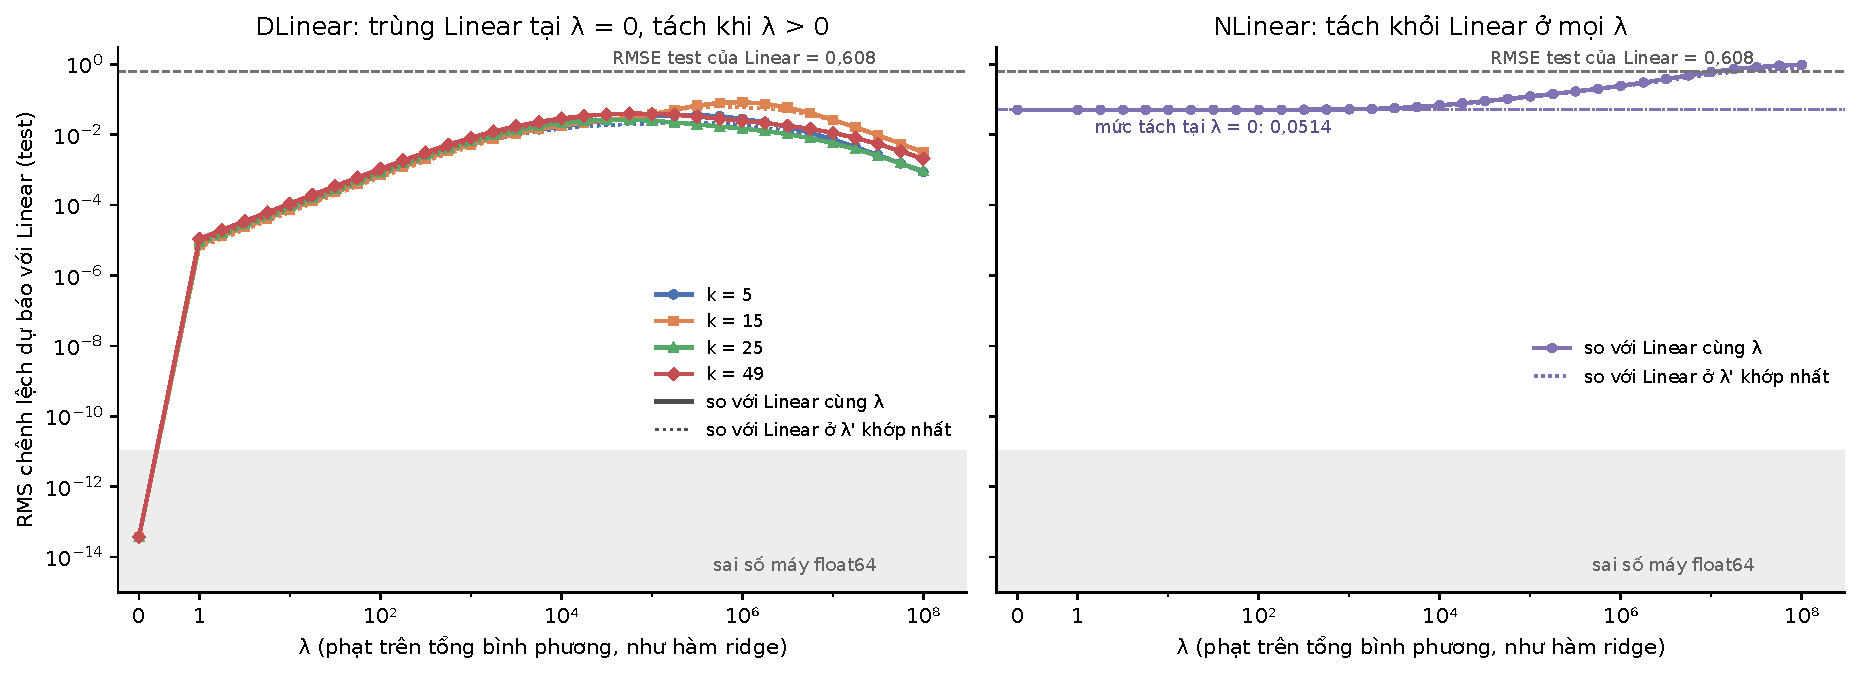
\includegraphics[width=\linewidth]{H1_three_predictions.pdf}
\begin{figurecardcaptionaivn}
\capfig{Hình H1: RMS chênh lệch dự báo trên test giữa DLinear (trái, bốn kernel $k$) hoặc NLinear (phải) và Linear, theo $\lambda$; ETTh1, $H = 96$, nghiệm tối ưu. Nét liền: so với Linear cùng $\lambda$; nét chấm: so với Linear ở $\lambda'$ khớp nhất. Dải xám: sai số máy float64. Đường đứt: RMSE test của Linear (\nmBTwoLinRmseTest).}\label{fig:h1}
\end{figurecardcaptionaivn}
\end{figure}

\paragraph{Độ lớn thực tế trên toàn bộ ma trận.} Hai loại tách có độ lớn rất khác nhau ở mức phạt mà val chọn (\tabref{tab:b3}).
\begin{itemize}
    \item \textbf{DLinear so với Linear: nhỏ.} Trên 12 cặp (dataset, $H$), MSE test của DLinear và Linear ở $\lambda^*$ (mục tiêu MSE) chênh nhau không quá \nmBThreeDLinMinusLinAbsMax. Trên mọi tổ hợp mục tiêu và metric (\nmBThreeDLinMinusLinAllCount{} cặp), mức chênh không quá \nmBThreeDLinMinusLinAllAbsMax.
    \item \textbf{NLinear so với Linear: phụ thuộc dataset.} NLinear $-$ Linear trên MSE test (mục tiêu MSE, theo $H$ từ nhỏ đến lớn về độ lớn) là \nmBThreeNLinMinusLinETThOneRange{} ở ETTh1, \nmBThreeNLinMinusLinETThTwoRange{} ở ETTh2 và \nmBThreeNLinMinusLinETTmOneRange{} ở ETTm1. Trên số liệu này, ràng buộc tổng hàng bằng $1$ có lợi rõ trên ETTh2 (tăng theo $H$) và ở ETTh1 $H = 720$, nhỏ ở các ô ETTh1 còn lại, và hơi bất lợi trên ETTm1.
\end{itemize}

\paragraph{ETTh1, $H = 720$.} Trong Bảng~2 của bài gốc, DLinear tốt hơn Linear rõ nhất ở ô này: \nmBOneETThOneHSevenTwoZeroDLinearPub{} so với \nmBOneETThOneHSevenTwoZeroLinearPub{} (chênh \nmCThreeETThOneHSevenTwoZeroPubD). Tại nghiệm tối ưu, hai mô hình cho \nmBThreeETThOneHSevenTwoZeroDLinearMSEMse{} và \nmBThreeETThOneHSevenTwoZeroLinearMSEMse. Với SGD của repo (20 seed, lr gốc), Linear cho \nmBOneETThOneHSevenTwoZeroLinearMean{} $\pm$ \nmBOneETThOneHSevenTwoZeroLinearSd{} và DLinear cho \nmBOneETThOneHSevenTwoZeroDLinearMean{} $\pm$ \nmBOneETThOneHSevenTwoZeroDLinearSd. Chênh DLinear $-$ Linear là \nmCThreeETThOneHSevenTwoZeroDTest{} với CI $95\%$ [\nmCThreeETThOneHSevenTwoZeroDTestLo; \nmCThreeETThOneHSevenTwoZeroDTestHi], tức không phát hiện khác biệt. Số công bố của Linear (\nmBOneETThOneHSevenTwoZeroLinearPub) thuộc đuôi trên của phân phối theo seed (\secref{sec:rq3}). ETTh2, $H = 720$ cho cùng kết luận: chênh trong bài là \nmCThreeETThTwoHSevenTwoZeroPubD, còn trung bình theo seed là \nmCThreeETThTwoHSevenTwoZeroDTest{} [\nmCThreeETThTwoHSevenTwoZeroDTestLo; \nmCThreeETThTwoHSevenTwoZeroDTestHi].

\paragraph{DLinear so với Linear khi huấn luyện bằng SGD.} \tabref{tab:c3} so DLinear $-$ Linear trên MSE test khi cả hai được huấn luyện bằng SGD. Với lr gốc, DLinear tốt hơn có ý nghĩa (CI Welch nằm hẳn dưới $0$, trên cả val lẫn test) ở \nmCThreeDLinBetterBothCount/12 ô, cả bốn đều trên ETTm1, với chênh \nmCThreeSigDTestRange. Ở các ô đó, chênh tương ứng của nghiệm dạng đóng nhỏ hơn hẳn (cột cuối). Khi tinh chỉnh lr cho cả hai mô hình (\secref{sec:method-sgd}), không còn ô nào có khác biệt ý nghĩa (\nmTunedCThreeDLinBetterCount/12). Ở ETTm1, chênh còn \nmTunedCThreeETTmOneDTestRange{} và mọi CI chứa $0$. Với lr gốc trên đúng 15 seed mới, cả \nmTunedCThreeXOneETTmOneTestCount/4 ô ETTm1 vẫn có ý nghĩa trên test. Vì vậy việc mất ý nghĩa là do lr, không do bớt seed. Không ô nào có Linear tốt hơn DLinear có ý nghĩa.

\begin{center}
\small
% Tự động sinh bởi scripts/report/make_tables.py từ results/. KHÔNG SỬA TAY.
\begin{tabular}{@{}lr l l l r@{}}
\toprule
Dataset & $H$ & lr gốc, 20 seed & lr tinh chỉnh, 15 seed & lr (Linear / DLinear) & dạng đóng \\
\midrule
ETTh1 & 96 & $-$0{,}0020 [$-$0{,}0075; 0{,}0036] & +0{,}0003 [$-$0{,}0040; 0{,}0046] & $\times$4 / $\times$1 & $-$0{,}0004 \\
ETTh1 & 192 & $-$0{,}0105 [$-$0{,}0227; 0{,}0017] & $-$0{,}0145 [$-$0{,}0307; 0{,}0016] & $\times$8 / $\times$2 & $-$0{,}0004 \\
ETTh1 & 336 & +0{,}0020 [$-$0{,}0150; 0{,}0190] & $-$0{,}0043 [$-$0{,}0224; 0{,}0138] & $\times$1 / $\times$0{,}5 & $-$0{,}0006 \\
ETTh1 & 720 & +0{,}0033 [$-$0{,}0210; 0{,}0276] & $-$0{,}0096 [$-$0{,}0238; 0{,}0046] & $\times$0{,}5 / $\times$8 & $-$0{,}0004 \\
\addlinespace[3pt]
ETTh2 & 96 & $-$0{,}0055 [$-$0{,}0148; 0{,}0037] & $-$0{,}0064 [$-$0{,}0182; 0{,}0054] & $\times$1 / $\times$1 & $-$0{,}0001 \\
ETTh2 & 192 & $-$0{,}0154 [$-$0{,}0383; 0{,}0075] & $-$0{,}0195 [$-$0{,}0459; 0{,}0069] & $\times$4 / $\times$0{,}5 & +0{,}0000 \\
ETTh2 & 336 & +0{,}0033 [$-$0{,}0122; 0{,}0187] & +0{,}0007 [$-$0{,}0170; 0{,}0184] & $\times$1 / $\times$1 & +0{,}0000 \\
ETTh2 & 720 & $-$0{,}0098 [$-$0{,}0444; 0{,}0249] & $-$0{,}0193 [$-$0{,}0700; 0{,}0314] & $\times$0{,}5 / $\times$1 & +0{,}0000 \\
\addlinespace[3pt]
ETTm1 & 96 & \textbf{$-$0{,}0040 [$-$0{,}0052; $-$0{,}0028]} & +0{,}0002 [$-$0{,}0017; 0{,}0022] & $\times$8 / $\times$2 & +0{,}0000 \\
ETTm1 & 192 & \textbf{$-$0{,}0032 [$-$0{,}0041; $-$0{,}0024]} & $-$0{,}0010 [$-$0{,}0028; 0{,}0008] & $\times$8 / $\times$2 & +0{,}0000 \\
ETTm1 & 336 & \textbf{$-$0{,}0038 [$-$0{,}0054; $-$0{,}0021]} & $-$0{,}0020 [$-$0{,}0073; 0{,}0033] & $\times$8 / $\times$4 & +0{,}0000 \\
ETTm1 & 720 & \textbf{$-$0{,}0047 [$-$0{,}0069; $-$0{,}0025]} & $-$0{,}0020 [$-$0{,}0058; 0{,}0017] & $\times$2 / $\times$2 & +0{,}0000 \\
\bottomrule
\end{tabular}

\end{center}
\begin{captionbelowboxaivn}
\captab{DLinear $-$ Linear, MSE test, huấn luyện bằng SGD. Trung bình theo seed, CI $95\%$ Welch; âm nghĩa là DLinear tốt hơn; \textbf{đậm}: DLinear tốt hơn có ý nghĩa trên test. Cột lr: mức đã chọn cho từng mô hình (bội của lr gốc). Cột cuối: cùng hiệu số với nghiệm dạng đóng MSE ở $\lambda^*$.}\label{tab:c3}
\end{captionbelowboxaivn}

\begin{guidelinebox}{Trả lời RQ1}
Tại nghiệm tối ưu, DLinear thu về đúng Linear khi không phạt, và chỉ tách khi có weight decay, qua metric $N^{-1}$ phụ thuộc kernel. NLinear là Linear có ràng buộc tổng hàng nên tách ở mọi $\lambda$. Ở $\lambda^*$ chọn trên val, khác biệt DLinear $-$ Linear rất nhỏ trên test. Khác biệt NLinear $-$ Linear thì phụ thuộc dữ liệu: lớn trên ETTh2, nhỏ trên ETTh1 (trừ $H = 720$) và ETTm1. Lợi thế của DLinear so với Linear trong các bảng công bố không xuất hiện ở nghiệm tối ưu. Với SGD, nó chỉ xuất hiện ở ETTm1 khi dùng lr gốc, và biến mất khi tinh chỉnh lr.
\end{guidelinebox}

% ---------------------------------------------------------------------------
\subsection{RQ2: hàm mục tiêu và outlier}
\label{sec:rq2}

\tabref{tab:b3} là bản gọn của bảng B3. Bản đủ, gồm $\lambda = 0$, $\lambda^*$ và $\delta$, nằm ở Phụ lục~\ref{app:tables}. MSE test được báo ở $\lambda^*_{\mathrm{MSE}}$, MAE test ở $\lambda^*_{\mathrm{MAE}}$ (\secref{sec:method-lambda}), và Huber dùng $\dmad$.

{\small
% Tự động sinh bởi scripts/report/make_tables.py từ results/. KHÔNG SỬA TAY.
\begin{longtable}{@{}llr rrr rrr@{}}
\toprule
 & & & \multicolumn{3}{c}{MSE test ở $\lambda^*_{\mathrm{MSE}}$} & \multicolumn{3}{c}{MAE test ở $\lambda^*_{\mathrm{MAE}}$} \\
\cmidrule(lr){4-6}\cmidrule(l){7-9}
Dataset & Mô hình & $H$ & MSE & MAE & Huber & MSE & MAE & Huber \\
\midrule
\endhead
ETTh1 & Linear & 96 & 0{,}3702 & \textbf{0{,}3653} & 0{,}3658 & 0{,}3915 & \textbf{0{,}3833} & 0{,}3852 \\
ETTh1 & Linear & 192 & 0{,}4040 & 0{,}4031 & \textbf{0{,}4025} & 0{,}4126 & \textbf{0{,}4074} & 0{,}4082 \\
ETTh1 & Linear & 336 & 0{,}4324 & 0{,}4302 & \textbf{0{,}4296} & 0{,}4340 & \textbf{0{,}4275} & 0{,}4285 \\
ETTh1 & Linear & 720 & 0{,}4701 & \textbf{0{,}4553} & 0{,}4624 & 0{,}4878 & \textbf{0{,}4747} & 0{,}4767 \\
\addlinespace[2pt]
ETTh1 & DLinear & 96 & 0{,}3698 & \textbf{0{,}3647} & 0{,}3652 & 0{,}3914 & \textbf{0{,}3832} & 0{,}3851 \\
ETTh1 & DLinear & 192 & 0{,}4036 & \textbf{0{,}4014} & 0{,}4017 & 0{,}4125 & \textbf{0{,}4074} & 0{,}4080 \\
ETTh1 & DLinear & 336 & 0{,}4317 & 0{,}4296 & \textbf{0{,}4290} & 0{,}4340 & \textbf{0{,}4272} & 0{,}4285 \\
ETTh1 & DLinear & 720 & 0{,}4697 & \textbf{0{,}4549} & 0{,}4620 & 0{,}4879 & \textbf{0{,}4746} & 0{,}4766 \\
\addlinespace[2pt]
ETTh1 & NLinear & 96 & 0{,}3695 & \textbf{0{,}3638} & 0{,}3656 & 0{,}3913 & \textbf{0{,}3839} & 0{,}3860 \\
ETTh1 & NLinear & 192 & 0{,}4027 & 0{,}4026 & \textbf{0{,}4024} & 0{,}4110 & \textbf{0{,}4075} & 0{,}4084 \\
ETTh1 & NLinear & 336 & \textbf{0{,}4261} & 0{,}4290 & 0{,}4307 & 0{,}4260 & \textbf{0{,}4237} & 0{,}4246 \\
ETTh1 & NLinear & 720 & 0{,}4329 & \textbf{0{,}4282} & 0{,}4329 & 0{,}4505 & \textbf{0{,}4454} & 0{,}4468 \\
\addlinespace[2pt]
\midrule
ETTh2 & Linear & 96 & 0{,}3009 & \textbf{0{,}2779} & 0{,}2818 & 0{,}3649 & \textbf{0{,}3334} & 0{,}3410 \\
ETTh2 & Linear & 192 & 0{,}3966 & \textbf{0{,}3531} & 0{,}3600 & 0{,}4273 & \textbf{0{,}3855} & 0{,}3945 \\
ETTh2 & Linear & 336 & 0{,}4853 & \textbf{0{,}4106} & 0{,}4220 & 0{,}4835 & \textbf{0{,}4296} & 0{,}4400 \\
ETTh2 & Linear & 720 & 0{,}7404 & \textbf{0{,}5893} & 0{,}6277 & 0{,}6115 & \textbf{0{,}5335} & 0{,}5541 \\
\addlinespace[2pt]
ETTh2 & DLinear & 96 & 0{,}3008 & \textbf{0{,}2778} & 0{,}2817 & 0{,}3649 & \textbf{0{,}3333} & 0{,}3410 \\
ETTh2 & DLinear & 192 & 0{,}3966 & \textbf{0{,}3531} & 0{,}3600 & 0{,}4273 & \textbf{0{,}3855} & 0{,}3945 \\
ETTh2 & DLinear & 336 & 0{,}4853 & \textbf{0{,}4106} & 0{,}4220 & 0{,}4835 & \textbf{0{,}4296} & 0{,}4400 \\
ETTh2 & DLinear & 720 & 0{,}7403 & \textbf{0{,}5892} & 0{,}6276 & 0{,}6115 & \textbf{0{,}5335} & 0{,}5541 \\
\addlinespace[2pt]
ETTh2 & NLinear & 96 & \textbf{0{,}2717} & 0{,}2764 & 0{,}2756 & 0{,}3342 & 0{,}3307 & \textbf{0{,}3306} \\
ETTh2 & NLinear & 192 & \textbf{0{,}3336} & 0{,}3447 & 0{,}3427 & 0{,}3754 & 0{,}3756 & \textbf{0{,}3744} \\
ETTh2 & NLinear & 336 & \textbf{0{,}3581} & 0{,}3760 & 0{,}3727 & \textbf{0{,}3997} & 0{,}4028 & 0{,}4008 \\
ETTh2 & NLinear & 720 & 0{,}3924 & 0{,}3926 & \textbf{0{,}3912} & 0{,}4341 & \textbf{0{,}4242} & 0{,}4251 \\
\addlinespace[2pt]
\midrule
ETTm1 & Linear & 96 & 0{,}2992 & \textbf{0{,}2929} & 0{,}2953 & 0{,}3427 & \textbf{0{,}3331} & 0{,}3362 \\
ETTm1 & Linear & 192 & 0{,}3340 & \textbf{0{,}3322} & 0{,}3327 & 0{,}3637 & \textbf{0{,}3553} & 0{,}3578 \\
ETTm1 & Linear & 336 & 0{,}3683 & \textbf{0{,}3658} & 0{,}3661 & 0{,}3843 & \textbf{0{,}3759} & 0{,}3782 \\
ETTm1 & Linear & 720 & 0{,}4232 & 0{,}4216 & \textbf{0{,}4210} & 0{,}4181 & \textbf{0{,}4101} & 0{,}4120 \\
\addlinespace[2pt]
ETTm1 & DLinear & 96 & 0{,}2992 & \textbf{0{,}2929} & 0{,}2952 & 0{,}3427 & \textbf{0{,}3331} & 0{,}3362 \\
ETTm1 & DLinear & 192 & 0{,}3339 & \textbf{0{,}3319} & 0{,}3326 & 0{,}3637 & \textbf{0{,}3553} & 0{,}3578 \\
ETTm1 & DLinear & 336 & 0{,}3683 & \textbf{0{,}3655} & 0{,}3660 & 0{,}3843 & \textbf{0{,}3759} & 0{,}3782 \\
ETTm1 & DLinear & 720 & 0{,}4232 & 0{,}4213 & \textbf{0{,}4208} & 0{,}4181 & \textbf{0{,}4101} & 0{,}4121 \\
\addlinespace[2pt]
ETTm1 & NLinear & 96 & 0{,}3004 & \textbf{0{,}2937} & 0{,}2964 & 0{,}3426 & \textbf{0{,}3337} & 0{,}3367 \\
ETTm1 & NLinear & 192 & 0{,}3356 & \textbf{0{,}3335} & 0{,}3345 & 0{,}3634 & \textbf{0{,}3563} & 0{,}3585 \\
ETTm1 & NLinear & 336 & 0{,}3703 & \textbf{0{,}3685} & 0{,}3691 & 0{,}3834 & \textbf{0{,}3770} & 0{,}3790 \\
ETTm1 & NLinear & 720 & \textbf{0{,}4262} & 0{,}4270 & 0{,}4264 & 0{,}4157 & \textbf{0{,}4113} & 0{,}4126 \\
\addlinespace[2pt]
\bottomrule
\end{longtable}

}
\begin{captionbelowboxaivn}
\captab{Bảng B3 (bản gọn): sai số test tại nghiệm tối ưu của ba mục tiêu huấn luyện (cột MSE, MAE, Huber trong mỗi nhóm). \textbf{Đậm}: thấp nhất giữa ba mục tiêu trong cùng (dataset, $H$, mô hình, metric).}\label{tab:b3}
\end{captionbelowboxaivn}

\paragraph{MAE so với MSE.} Huấn luyện bằng MAE cho MSE test thấp hơn huấn luyện bằng MSE ở \nmBThreeMaeBeatsMseTotalCount/\nmBThreeCellCount{} ô. Với Linear và DLinear, điều này đúng ở cả 4 horizon của cả ba dataset. Chênh lớn nhất ở ETTh2 (\nmBThreeMaeGainETThTwoLinDLinRange), nhỏ ở ETTh1 (\nmBThreeMaeGainETThOneLinDLinRange) và ETTm1 (\nmBThreeMaeGainETTmOneLinDLinRange). Với NLinear, MAE tốt hơn ở \nmBThreeMaeBeatsMseETThOneNLinearCount/4 horizon của ETTh1 và \nmBThreeMaeBeatsMseETTmOneNLinearCount/4 của ETTm1, nhưng kém hơn ở cả 4 horizon của ETTh2 (chênh \nmBThreeMaeGainETThTwoNLinearRange). Theo MSE test, mục tiêu tốt nhất trong ô là MAE ở \nmBThreeBestMAEMseCount{} ô, Huber ở \nmBThreeBestHuberMseCount{} và MSE ở \nmBThreeBestMSEMseCount. Theo MAE test, các con số là \nmBThreeBestMAEMaeCount{} / \nmBThreeBestHuberMaeCount{} / \nmBThreeBestMSEMaeCount. Trên ETTh2, khoảng một nửa lợi thế của MAE với Linear ở $H \ge 336$ đến từ các đoạn cảm biến bị kẹt (\secref{sec:etth2}).

\paragraph{Vị trí của Huber.} Huber đứng giữa MSE và MAE ở \nmBThreeHuberRankTwoMseCount/\nmBThreeCellCount{} ô theo MSE test và \nmBThreeHuberRankTwoMaeCount/\nmBThreeCellCount{} theo MAE test. So với $\delta = 1$ cố định của các phiên trước, $\dmad$ cho MSE test thấp hơn ở \nmDeltaMadBetterMseCount/\nmBThreeCellCount{} ô và MAE test thấp hơn ở \nmDeltaMadBetterMaeCount/\nmBThreeCellCount. Lợi lớn nhất ở ETTh2 Linear $H = 720$ (MSE test \nmDeltaETThTwoLinearHSevenTwoZeroOne{} $\to$ \nmDeltaETThTwoLinearHSevenTwoZeroMad), nơi MAE vượt xa MSE.

\paragraph{Độ nhạy theo $\delta$.} \figref{fig:h4} quét $\delta \in \{0{,}5;\ 1;\ 2;\ 4\} \times \dmad$ trên 6 ô. MAE test tăng đơn điệu theo $\delta$ ở \nmDeltaSensMaeMonotoneCount/6 ô: $\delta$ nhỏ đưa Huber về MAE. Huber đứng hạng 2 ở \nmDeltaSensRankTwoCount/\nmDeltaSensCount{} trường hợp (ô, metric, $\delta$), kể cả $\delta = 1$. Giá trị tuyệt đối nhạy với $\delta$ ở ETTh2 Linear $H = 720$ (MSE test \nmDeltaSensETThTwoLinMseRange), gần hết khoảng giữa MAE và MSE. Ở ETTh1, biên độ chỉ \nmDeltaSensETThOneAmpRange.

\begin{figure}[H]
\centering
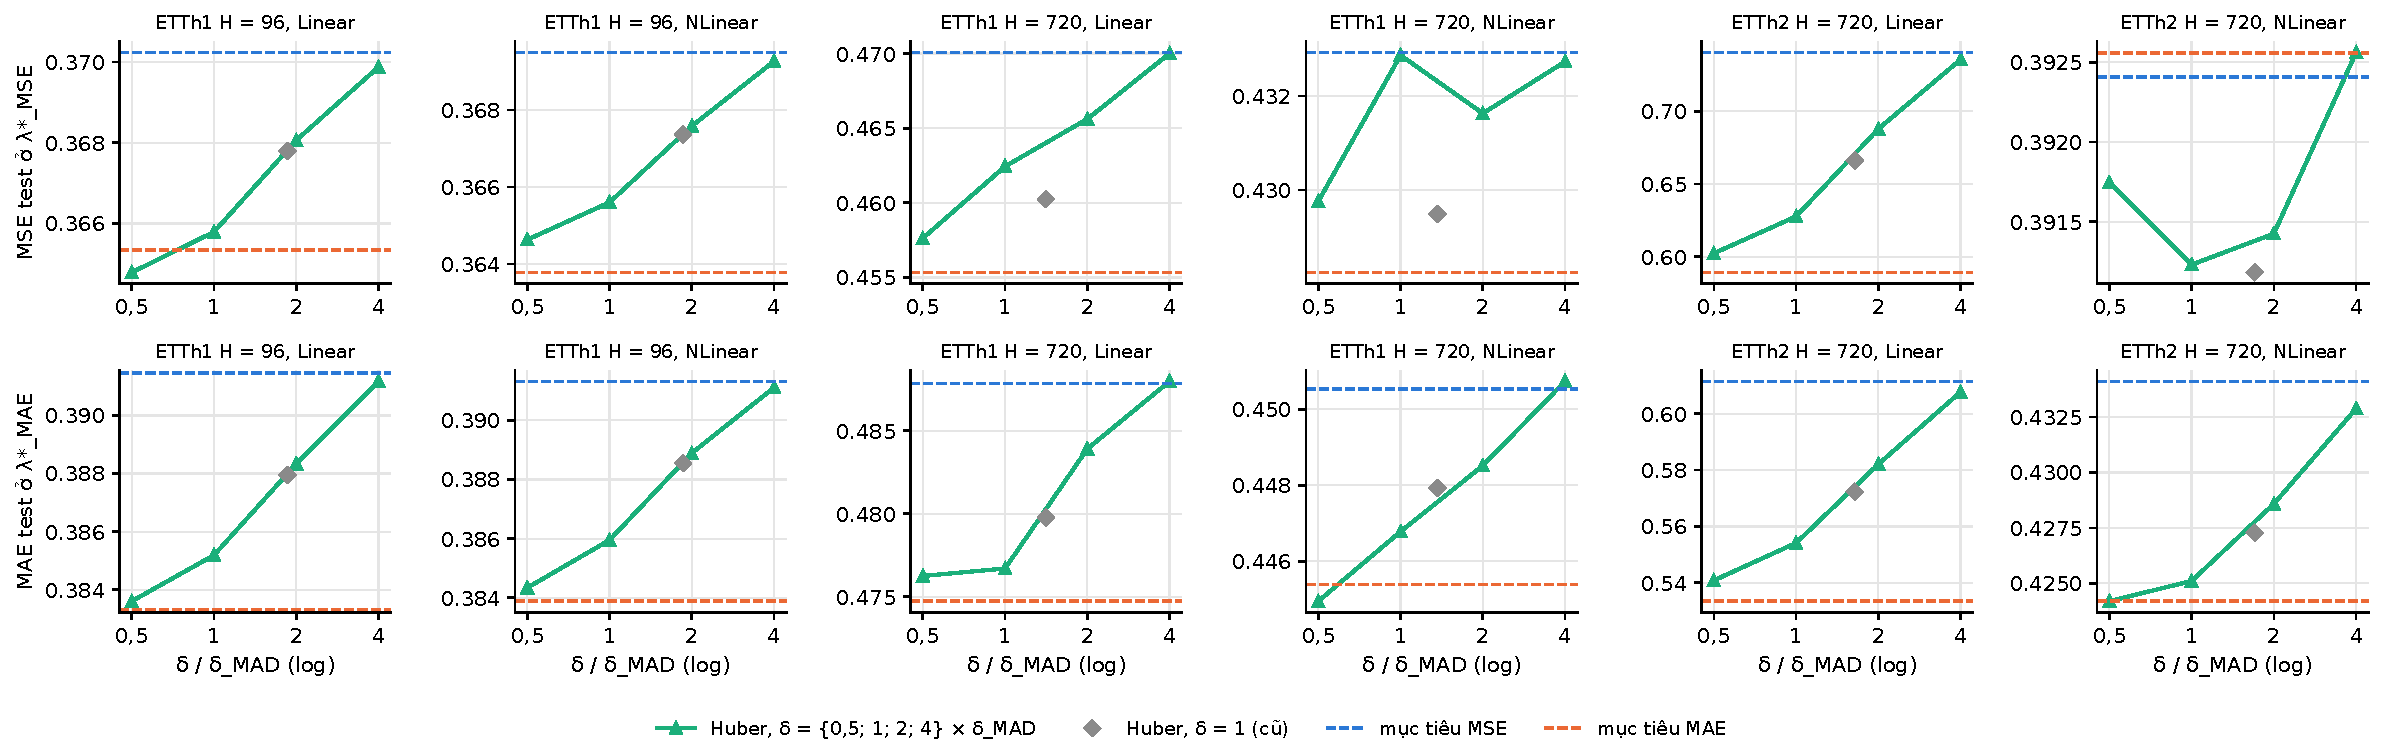
\includegraphics[width=\linewidth]{H4_delta_sensitivity.pdf}
\begin{figurecardcaptionaivn}
\capfig{Hình H4: độ nhạy của Huber theo $\delta$. Trục hoành $\delta/\dmad$ (log); hình thoi xám: $\delta = 1$ cố định. Đường đứt: mục tiêu MSE (xanh) và MAE (cam). Hàng trên: MSE test ở $\lambda^*_{\mathrm{MSE}}$; hàng dưới: MAE test ở $\lambda^*_{\mathrm{MAE}}$.}\label{fig:h4}
\end{figurecardcaptionaivn}
\end{figure}

\paragraph{Outlier chỉ ở đích.} Khi cộng $\pm 10$ độ lệch chuẩn vào $1\%$ hoặc $10\%$ phần tử đích của train ETTh1 (đầu vào giữ nguyên), MSE test của MAE và Huber đổi không quá \nmOutTargetRobustAbsMax. Trong khi đó, MSE test của mục tiêu MSE tăng tới \nmOutTargetMSEMax{} (nét đứt trong \figref{fig:h2}). Đây là hành vi mà lý thuyết hồi quy bền vững dự đoán.

\paragraph{Outlier trong chuỗi.} Khi outlier nằm trong chuỗi, tức xuất hiện cả ở đầu vào, thứ hạng đổi theo tỷ lệ (\figref{fig:h2}, nét liền; bảng đầy đủ ở Phụ lục~\ref{app:tables}). Ở $1\%$, MAE tốt nhất theo MSE test ở \nmOutSeriesBestMAEROneCount/8 ô (Linear, NLinear $\times$ 4 horizon). Ở $5\%$, MSE tốt nhất ở \nmOutSeriesBestMSERFiveCount/8, và ở $10\%$ là \nmOutSeriesBestMSEROneZeroCount/8. Mức suy giảm MSE test từ $0$ đến $10\%$ là \nmOutSeriesDegMSERange{} với MSE, \nmOutSeriesDegHuberRange{} với Huber và \nmOutSeriesDegMAERange{} với MAE. Thứ tự MSE $<$ Huber $<$ MAE đúng ở \nmOutSeriesDegOrderCount/8 ô. Độ lệch theo vị trí outlier (Linear, $H = 96$, $10\%$, seed 2026--2028) là \nmOutSeedSpreadRange, cùng cỡ khác biệt giữa MSE và Huber.

\begin{figure}[H]
\centering
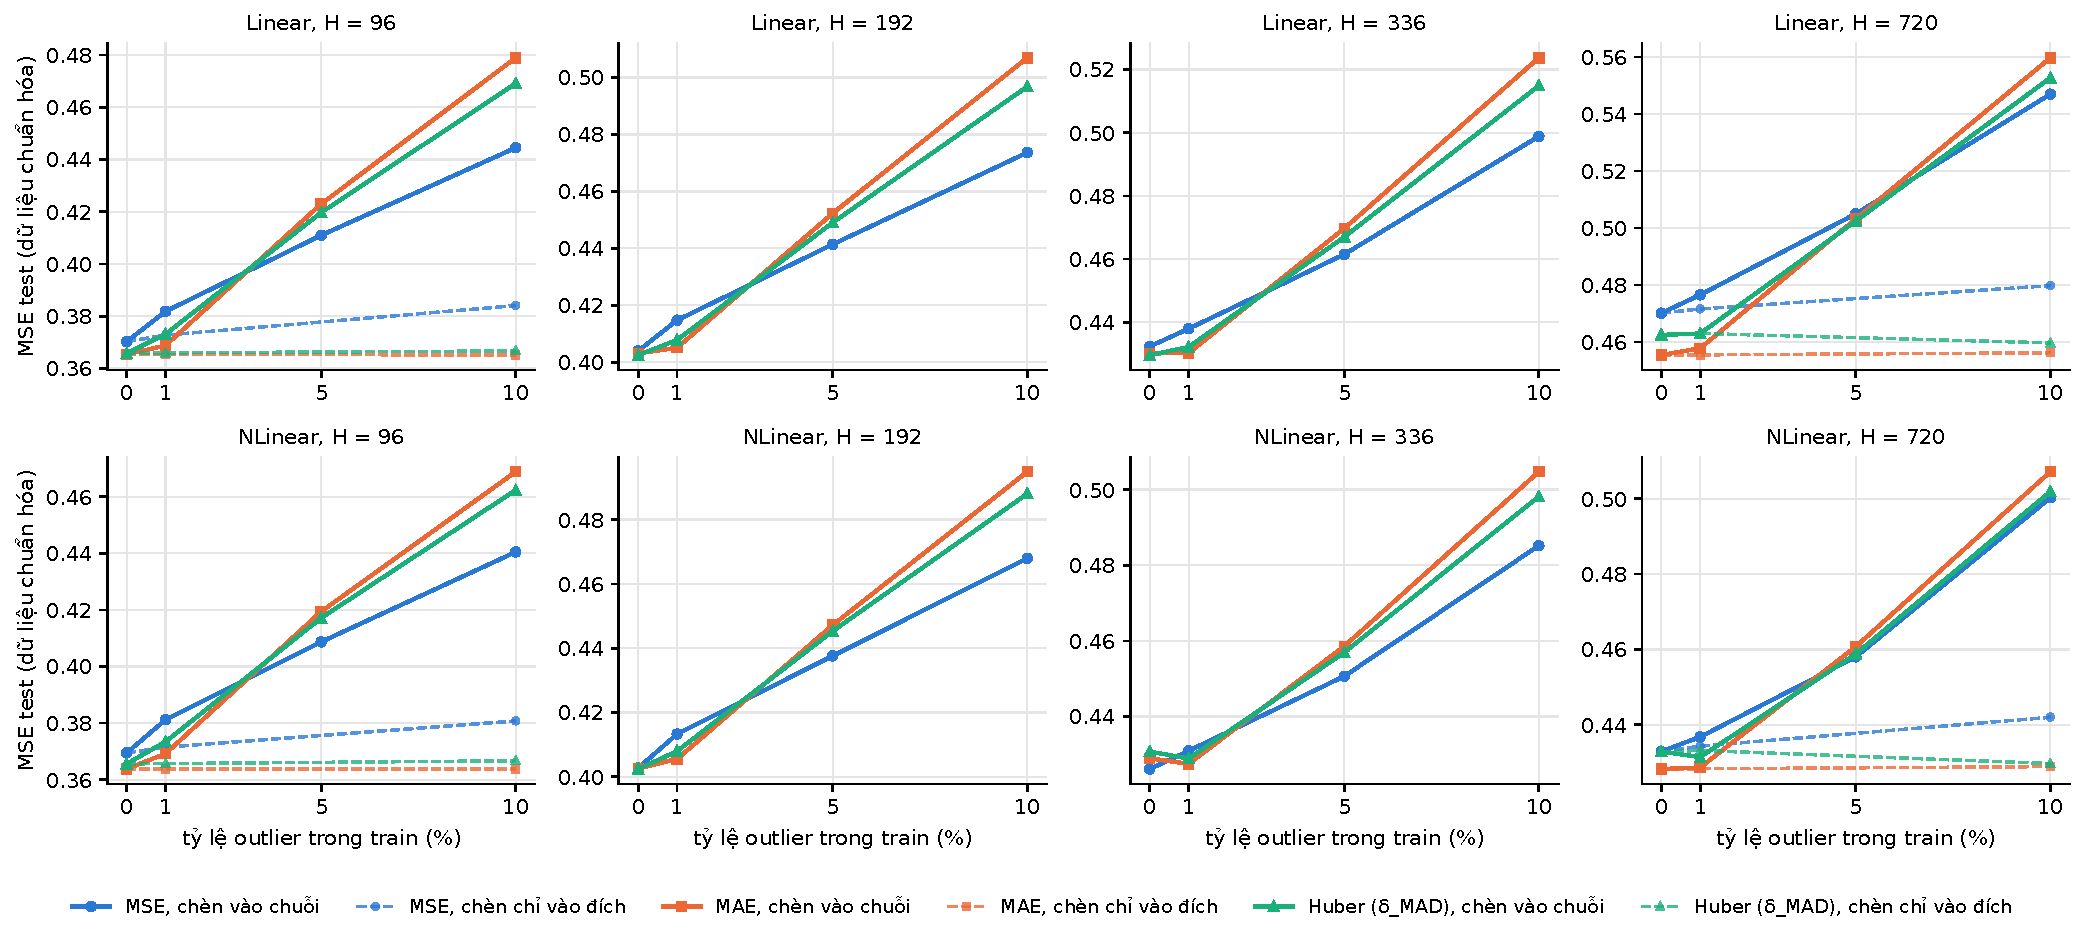
\includegraphics[width=\linewidth]{H2_outlier_mse.pdf}
\begin{figurecardcaptionaivn}
\capfig{Hình H2: MSE test theo tỷ lệ outlier trong train, ETTh1, outlier $\pm 10$ độ lệch chuẩn, seed 2026; $\lambda^*$ chọn theo MSE val sạch; Huber dùng $\dmad$ của chính tập train đã chèn. Nét liền: chèn vào chuỗi ($0$, $1$, $5$, $10\%$); nét đứt: chèn chỉ vào đích ($0$, $1$, $10\%$, chỉ $H = 96, 720$). Bản theo MAE test ở Phụ lục~\ref{app:tables}.}\label{fig:h2}
\end{figurecardcaptionaivn}
\end{figure}

\paragraph{Độ lớn outlier.} \figref{fig:h5} lặp lại thí nghiệm với outlier nhỏ hơn ($3\sigma$, $5\sigma$) ở cùng vị trí, cho Linear trên ETTh1 với một seed.
\begin{itemize}
    \item Chèn vào chuỗi ở $10\%$, $3\sigma$: MAE vẫn tốt nhất ở cả hai horizon. Ở $H = 96$, ba mục tiêu suy giảm gần bằng nhau (MSE \nmMagHNineSixSeriesROneMThreeMSEDeg, MAE \nmMagHNineSixSeriesROneMThreeMAEDeg, Huber \nmMagHNineSixSeriesROneMThreeHuberDeg).
    \item Ở $10\%$, $5\sigma$, $H = 96$: ba mục tiêu chênh không quá \nmMagHNineSixFiveSpread, nhỏ hơn độ lệch theo seed. Ở $H = 720$, MAE vẫn tốt hơn MSE (\nmMagHSevenTwoZeroSeriesRTenMFiveMAE{} so với \nmMagHSevenTwoZeroSeriesRTenMFiveMSE).
    \item Ở $10\%$, $10\sigma$: MSE tốt nhất ở cả hai horizon.
    \item Chèn chỉ vào đích: MSE suy giảm gần tỷ lệ với độ lớn ($H = 96$, $10\%$: \nmMagTargetMSEDegMThree{} / \nmMagTargetMSEDegMFive{} / \nmMagTargetMSEDegMOneZero{} ở $3\sigma$ / $5\sigma$ / $10\sigma$), còn MAE và Huber gần như không đổi.
\end{itemize}
Như vậy, MAE và Huber chỉ mất lợi thế khi outlier vừa nhiều ($10\%$) vừa lớn (từ khoảng $5\sigma$) và nằm cả trong đầu vào.

\begin{figure}[H]
\centering
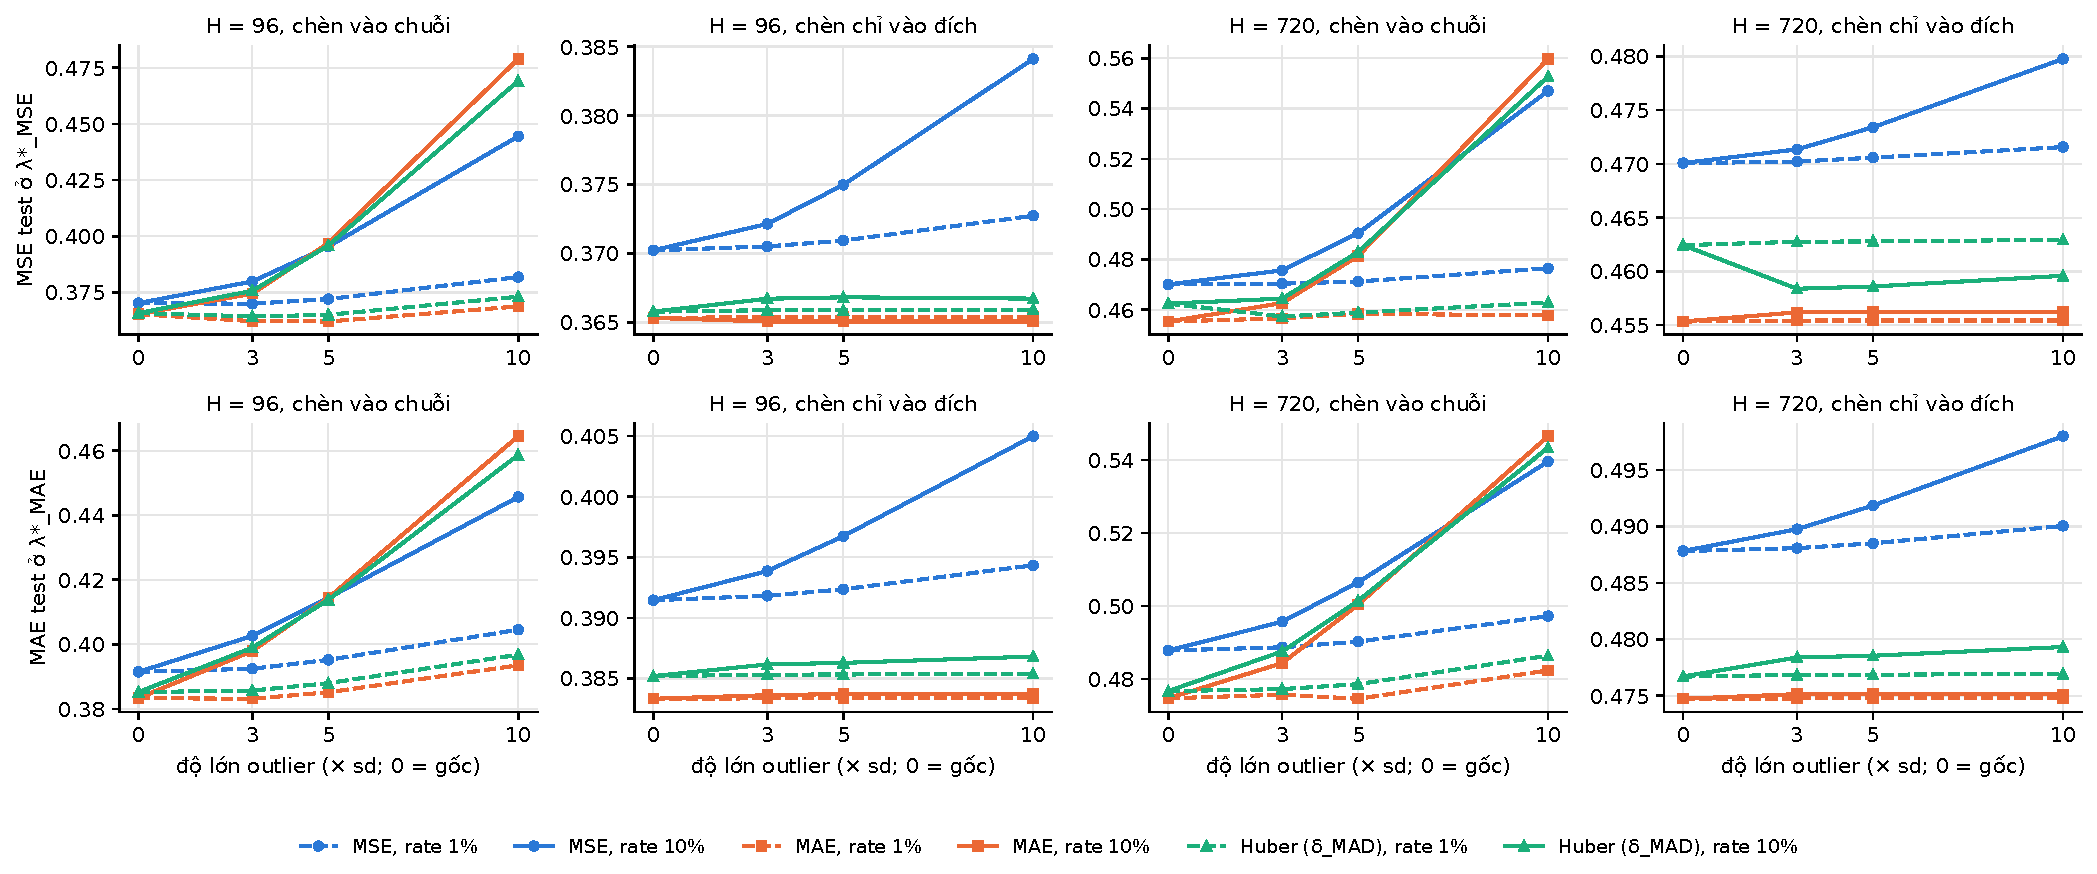
\includegraphics[width=\linewidth]{H5_outlier_magnitude.pdf}
\begin{figurecardcaptionaivn}
\capfig{Hình H5: sai số test theo độ lớn outlier, Linear, ETTh1, seed 2026, cùng vị trí outlier ở mọi độ lớn. Hàng trên: MSE test ở $\lambda^*_{\mathrm{MSE}}$; hàng dưới: MAE test ở $\lambda^*_{\mathrm{MAE}}$. Trục hoành: độ lớn (bội của độ lệch chuẩn; $0$ là dữ liệu gốc). Nét đứt: tỷ lệ $1\%$; nét liền: $10\%$.}\label{fig:h5}
\end{figurecardcaptionaivn}
\end{figure}

\begin{guidelinebox}{Trả lời RQ2}
Trên dữ liệu gốc, huấn luyện bằng MAE cho sai số test thấp hơn MSE ở phần lớn ô, kể cả khi đo bằng MSE. Lợi thế lớn nhất ở ETTh2, nơi một phần lợi thế đến từ các đoạn cảm biến bị kẹt; ngoại lệ là NLinear trên ETTh2. Huber với $\delta$ theo thang phần dư đứng giữa MSE và MAE ở phần lớn ô, và vị trí này ít nhạy với $\delta$. MAE và Huber bền vững với outlier chỉ nằm ở đích. Khi outlier nằm trong chuỗi, chúng vẫn tốt nhất ở tỷ lệ thấp hoặc độ lớn nhỏ, nhưng suy giảm nhanh hơn MSE khi outlier vừa nhiều vừa lớn.
\end{guidelinebox}

% ---------------------------------------------------------------------------
\subsection{RQ3: SGD so với nghiệm tối ưu}
\label{sec:rq3}

\paragraph{B1: tái lập số công bố.} \tabref{tab:b1} so SGD của repo (lr gốc, 20 seed) với số công bố. Số công bố nằm trong khoảng từ seed tốt nhất đến seed kém nhất ở \nmBOneInsideCount/36 ô. Ở cả \nmBOneOutsideCount{} ô còn lại, số công bố thấp hơn mọi seed. \nmBOneOutsideDLinearCount{} trong số đó là DLinear, và không ô nào là Linear. Pipeline của repo khác code gốc ở vài chi tiết, và tính tương đương mới chỉ được kiểm ở một ô (hạn chế~\ref{lim:pipeline}). Vì vậy chúng tôi không quy khoảng chênh ở các ô này cho may rủi theo seed. \figref{fig:h3} cho thấy toàn bộ phân phối theo seed cạnh nghiệm dạng đóng và số công bố.

\begin{center}
\footnotesize
% Tự động sinh bởi scripts/report/make_tables.py từ results/. KHÔNG SỬA TAY.
\begin{tabular}{@{}lr ll ll ll@{}}
\toprule
 & & \multicolumn{2}{c}{Linear} & \multicolumn{2}{c}{DLinear} & \multicolumn{2}{c}{NLinear} \\
\cmidrule(lr){3-4}\cmidrule(lr){5-6}\cmidrule(l){7-8}
Dataset & $H$ & SGD: TB $\pm$ sd & công bố & SGD: TB $\pm$ sd & công bố & SGD: TB $\pm$ sd & công bố \\
\midrule
ETTh1 & 96 & {,}786 $\pm$ {,}107 & {,}75 & {,}766 $\pm$ {,}057 & {,}75 & {,}779 $\pm$ {,}072 & {,}74 \\
ETTh1 & 192 & {,}250 $\pm$ {,}222 & {,}18 & {,}146 $\pm$ {,}152 & \textbf{{,}05}$^\dagger$ & {,}105 $\pm$ {,}106 & {,}08 \\
ETTh1 & 336 & {,}553 $\pm$ {,}189 & {,}79 & {,}573 $\pm$ {,}322 & {,}39 & {,}320 $\pm$ {,}042 & {,}29 \\
ETTh1 & 720 & {,}063 $\pm$ {,}363 & {,}24 & {,}096 $\pm$ {,}396 & \textbf{{,}72}$^\dagger$ & {,}363 $\pm$ {,}014 & {,}40 \\
\addlinespace[3pt]
ETTh2 & 96 & {,}968 $\pm$ {,}191 & {,}88 & {,}913 $\pm$ {,}060 & {,}89 & {,}770 $\pm$ {,}020 (10) & {,}77 \\
ETTh2 & 192 & {,}961 $\pm$ {,}472 & {,}77 & {,}807 $\pm$ {,}145 & {,}83 & {,}444 $\pm$ {,}041 (10) & {,}44 \\
ETTh2 & 336 & {,}496 $\pm$ {,}241 & {,}52 & {,}529 $\pm$ {,}242 & {,}48 & {,}804 $\pm$ {,}139 (10) & \textbf{{,}57}$^\dagger$ \\
ETTh2 & 720 & {,}967 $\pm$ {,}484 & {,}98 & {,}869 $\pm$ {,}592 & {,}05 & {,}058 $\pm$ {,}122 (10) & \textbf{{,}94}$^\dagger$ \\
\addlinespace[3pt]
ETTm1 & 96 & {,}057 $\pm$ {,}019 & {,}08 & {,}017 $\pm$ {,}018 & \textbf{{,}99}$^\dagger$ & {,}091 $\pm$ {,}042 & {,}06 \\
ETTm1 & 192 & {,}401 $\pm$ {,}012 & {,}40 & {,}369 $\pm$ {,}015 & \textbf{{,}35}$^\dagger$ & {,}436 $\pm$ {,}028 & {,}49 \\
ETTm1 & 336 & {,}769 $\pm$ {,}025 & {,}76 & {,}731 $\pm$ {,}027 & \textbf{{,}69}$^\dagger$ & {,}779 $\pm$ {,}022 & \textbf{{,}75}$^\dagger$ \\
ETTm1 & 720 & {,}336 $\pm$ {,}039 & {,}40 & {,}289 $\pm$ {,}028 & {,}25 & {,}346 $\pm$ {,}031 & {,}33 \\
\bottomrule
\end{tabular}

\end{center}
\begin{captionbelowboxaivn}
\captab{Bảng B1: MSE test của SGD (lr gốc; trung bình $\pm$ độ lệch chuẩn theo seed; 20 seed, số khác ghi trong ngoặc) và số công bố của LTSF-Linear. $^\dagger$\textbf{Đậm}: số công bố nằm ngoài khoảng [min, max] của các seed.}\label{tab:b1}
\end{captionbelowboxaivn}

\begin{figure}[H]
\centering
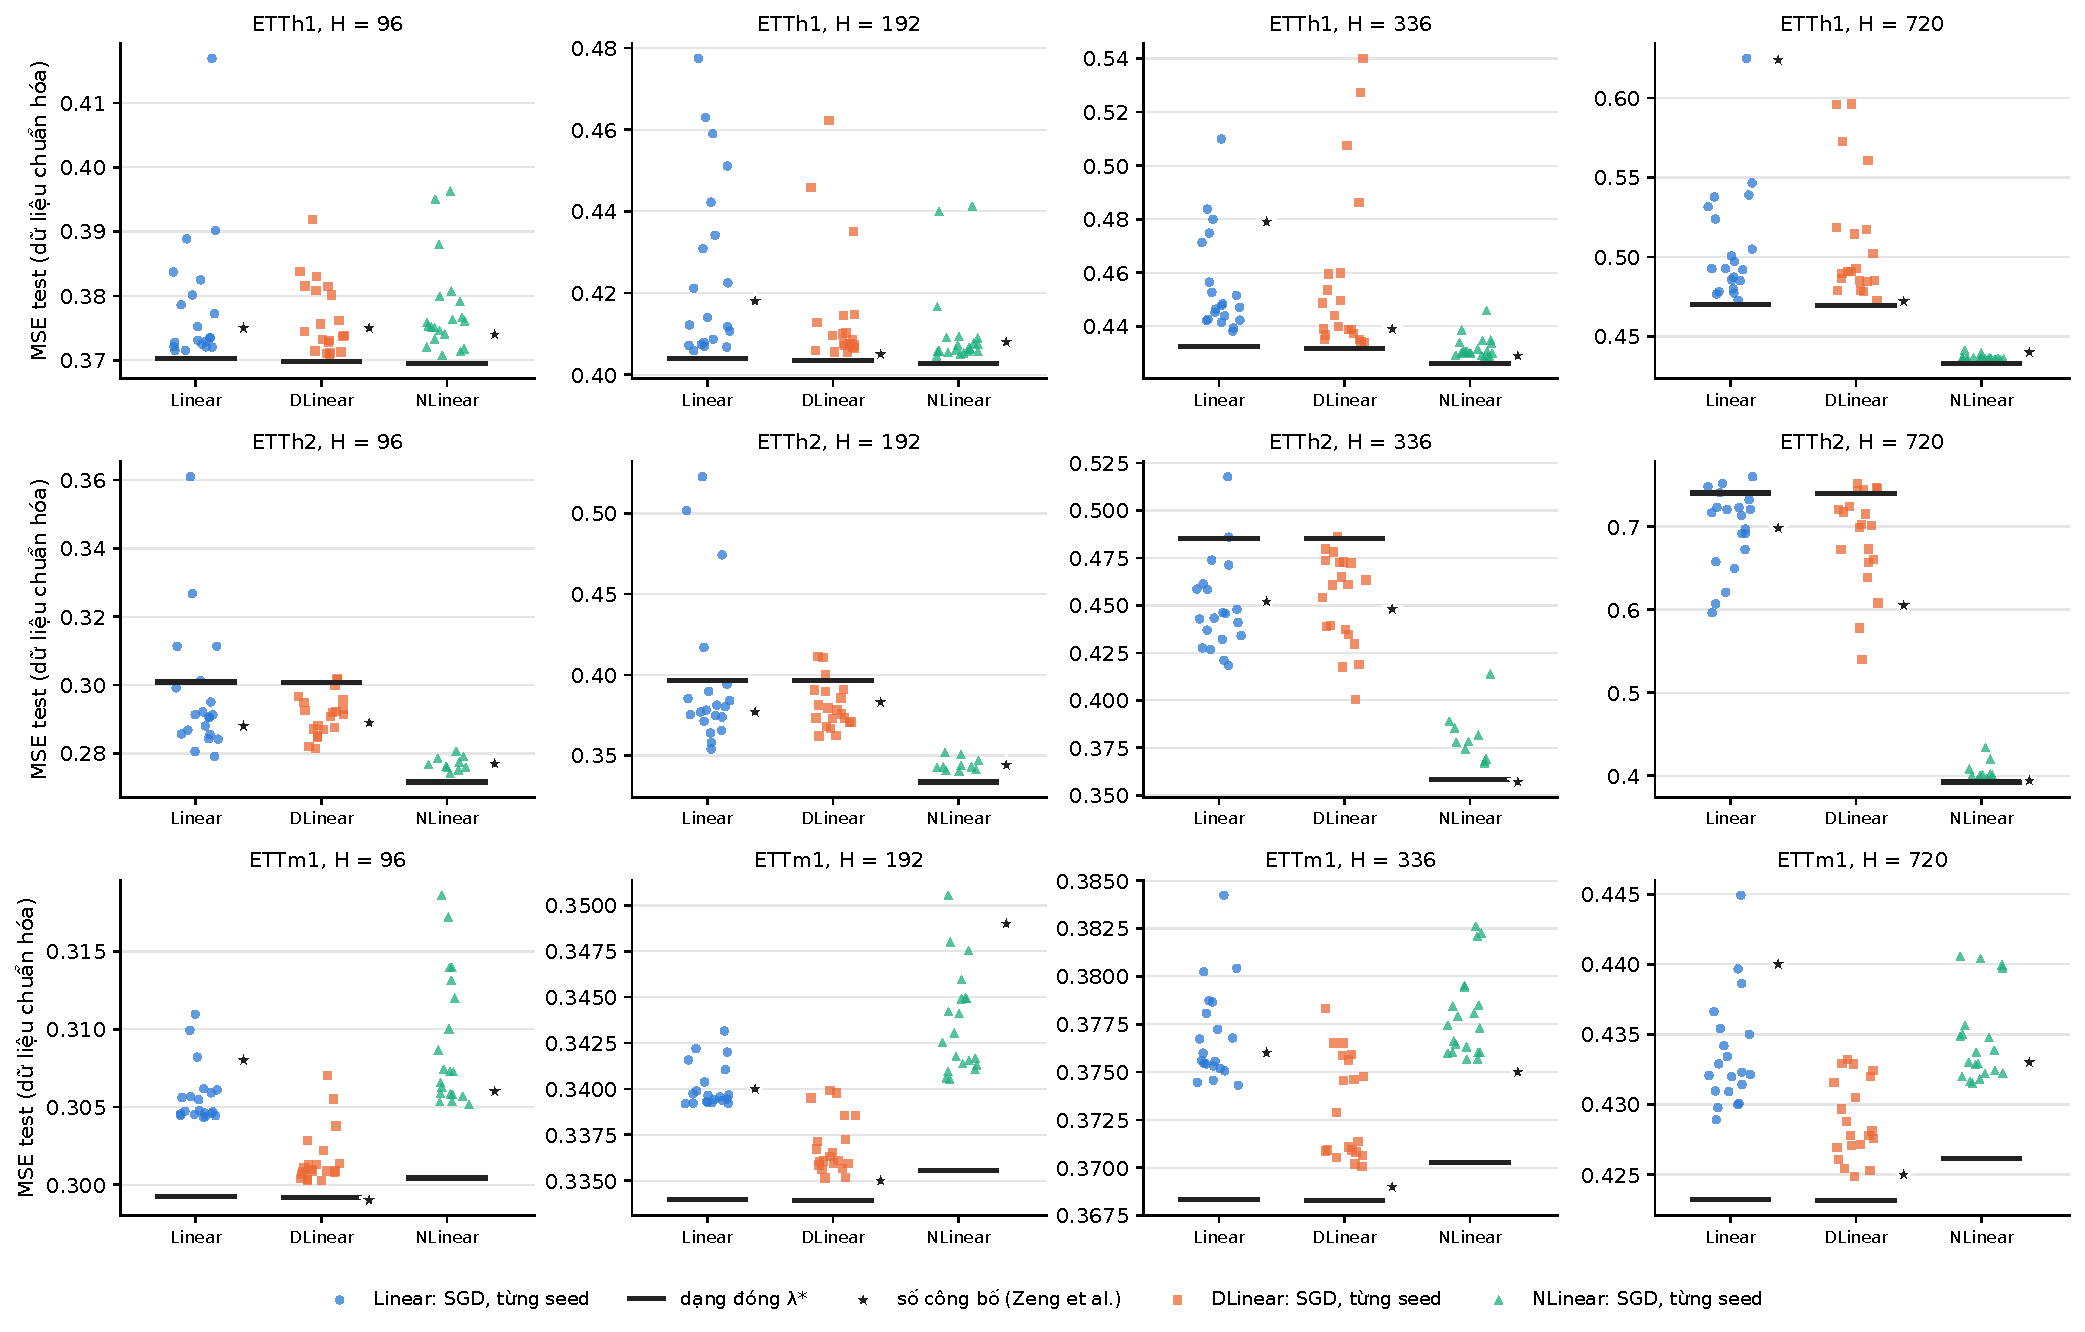
\includegraphics[width=\linewidth]{H3_sgd_vs_optimum.pdf}
\begin{figurecardcaptionaivn}
\capfig{Hình H3: MSE test của SGD theo seed (lr gốc; mỗi điểm một seed), so với nghiệm dạng đóng MSE ở $\lambda^*$ (vạch đen) và số công bố (dấu sao). Mỗi ô một (dataset, $H$), thang trục tung riêng.}\label{fig:h3}
\end{figurecardcaptionaivn}
\end{figure}

\paragraph{B4: khoảng cách SGD $-$ nghiệm dạng đóng.} \tabref{tab:b4} đếm nhãn theo quy tắc ở \tabref{tab:rule}; số liệu từng ô ở Phụ lục~\ref{app:tables}.
\begin{itemize}
    \item \textbf{lr gốc:} trên ETTh1 và ETTm1, SGD kém nghiệm dạng đóng trên test ở \nmBFourETThOneWorseCount/12 và \nmBFourETTmOneWorseCount/12 ô, với $\Delta$ test lần lượt \nmBFourETThOneDTestRange{} và \nmBFourETTmOneDTestRange. Trên ETTh1, SGD thường đạt val thấp hơn nhưng test cao hơn. Nhãn ``SGD tốt hơn thật'' chỉ có trên ETTh2, ở \nmBFourSgdBetterCount{} ô, đều với Linear hoặc DLinear.
    \item \textbf{lr tinh chỉnh:} lr được chọn trải đều trên các mức ($\times 0{,}5$: \nmTunedChosenZeroPointFiveCount{} ô; $\times 1$: \nmTunedChosenOneCount; $\times 2$: \nmTunedChosenTwoCount; $\times 4$: \nmTunedChosenFourCount; $\times 8$: \nmTunedChosenEightCount). \nmTunedLrEdgeCount/\nmTunedLrCellCount{} ô chọn mức ở đầu mút của khoảng đã thử. Lựa chọn cũng nhiễu: ở \nmTunedLrNoisyCount/\nmTunedLrCellCount{} ô, mức được chọn hơn mức thứ hai chưa tới một sai số chuẩn (hạn chế~\ref{lim:lr}).
    \item \textbf{Kết quả sau tinh chỉnh:} SGD vẫn kém nghiệm dạng đóng trên test ở \nmTunedWorseMeanCount/\nmTunedLrCellCount{} ô theo trung bình, \nmTunedWorseSigCount/\nmTunedLrCellCount{} ô có ý nghĩa. Trên ETTh1 và ETTm1, con số là \nmTunedHMOneWorseSigCount/\nmTunedHMOneCellCount{} ô có ý nghĩa, với $\Delta$ test \nmTunedHMOneDTestRange. Nhãn đổi ở \nmTunedChangedCount{} ô, trong đó \nmTunedChangedByLrCount{} ô do lr (phần còn lại do bớt seed). ``Dạng đóng tốt hơn thật'' giảm từ \nmTunedCfBetterXOneCount{} xuống \nmTunedCfBetterCount{} ô, chủ yếu chuyển thành ``SGD có dấu hiệu khớp val quá mức'': tinh chỉnh lr giúp SGD trên val nhưng không giúp trên test. ``SGD tốt hơn thật'' còn \nmTunedSgdBetterCount{} ô, vẫn chỉ trên ETTh2 với Linear hoặc DLinear.
\end{itemize}

\begin{center}
\small
% Tự động sinh bởi scripts/report/make_tables.py từ results/. KHÔNG SỬA TAY.
\begin{tabular}{@{}lrrr@{}}
\toprule
Nhãn & lr gốc, 20 seed & lr gốc, 15 seed mới & lr tinh chỉnh, 15 seed mới \\
\midrule
T1: SGD tốt hơn thật & 6 & 6 & 5 \\
T2: dạng đóng tốt hơn thật & 10 & 10 & 2 \\
T3: val khác test & 7 & 7 & 8 \\
T4: SGD khớp val quá mức & 12 & 11 & 17 \\
T5: dạng đóng khớp val quá mức & 0 & 0 & 0 \\
T6: không phân biệt được & 1 & 2 & 4 \\
\midrule
Tổng & 36 & 36 & 36 \\
\bottomrule
\end{tabular}

\end{center}
\begin{captionbelowboxaivn}
\captab{Bảng B4: số ô (trên 36) theo nhãn của quy tắc ba trường hợp, $\Delta = $ SGD $-$ dạng đóng MSE ở $\lambda^*$. Cột giữa: lr gốc trên đúng 15 seed mới (2026--2040), để tách phần thay đổi do lr khỏi phần do bớt seed.}\label{tab:b4}
\end{captionbelowboxaivn}

\paragraph{Các cơ chế đã loại trừ trên ETTh2.} Hiện tượng SGD tốt hơn nghiệm tối ưu trên cả val và test chỉ xuất hiện ở ETTh2, với Linear và DLinear. Chúng tôi đã kiểm và không thấy ủng hộ cho các giải thích sau:
\begin{itemize}
    \item SGD ngầm co trọng số về một điểm khác $0$. Tổng hàng của $\Weff$ do SGD học không gần $1$ hơn một cách nhất quán. Ridge co về dự báo trung bình hay dự báo lặp giá trị cuối gần như không đổi MSE test.
    \item Các đoạn cảm biến bị kẹt. Bỏ các cửa sổ hằng khỏi train giúp cả SGD lẫn nghiệm dạng đóng, và khoảng cách vẫn âm ở phần lớn ô (\secref{sec:etth2}).
    \item Dừng sớm của gradient descent. Trên Linear ETTh2 $H = 720$, gradient descent toàn batch từ $0$ hoặc từ khởi tạo của LTSF-Linear cho sai số val và test gần như trùng ridge ở $\lambda^*$, đúng như lý thuyết~\cite{ali2019continuous}. Adam toàn batch hòa trên val nhưng thắng trên test.
\end{itemize}
Kết quả không khớp mẫu nào đã đặt trước, nên chúng tôi không xác định được cơ chế (hạn chế~\ref{lim:etth2}).

\begin{guidelinebox}{Trả lời RQ3}
Với siêu tham số gốc, SGD kém nghiệm tối ưu trên test ở mọi ô của ETTh1 và ETTm1. Khoảng cách lớn hơn ở ETTh1 (\nmBFourETThOneDTestRange) so với ETTm1 (\nmBFourETTmOneDTestRange); theo bảng đầy đủ ở Phụ lục~\ref{app:tables}, với Linear và DLinear trên ETTh1 nó tăng theo horizon, còn với NLinear thì không. Tinh chỉnh learning rate trên val không đóng được khoảng cách này trên test: SGD vẫn kém ở \nmTunedWorseSigCount/36 ô (có ý nghĩa). Ngoại lệ duy nhất là ETTh2 với Linear và DLinear: ở đó SGD tốt hơn nghiệm tối ưu trên cả val và test, chưa rõ cơ chế. Số công bố (một lần chạy) nằm trong khoảng giữa seed tốt nhất và kém nhất ở \nmBOneInsideCount/36 ô. Các chênh lệch lớn giữa DLinear và Linear ở $H = 720$ trong bảng công bố không xuất hiện khi lấy trung bình theo seed.
\end{guidelinebox}

% ---------------------------------------------------------------------------
\subsection{ETTh2 và các đoạn cảm biến bị kẹt}
\label{sec:etth2}

ETTh2 chứa các đoạn mà ba kênh tải (MUFL, LUFL, LULL) giữ nguyên một giá trị trong thời gian dài, nhiều khả năng do cảm biến bị kẹt. Sau khi chia cửa sổ, \nmEThTwoConstTrainPctRange\% số cửa sổ train có đầu vào hoặc đích hằng. Mọi kết quả chính ở trên dùng dữ liệu gốc. Phần này là phân tích độ nhạy: bỏ các cửa sổ hằng khỏi train, giữ nguyên val và test.

\begin{itemize}
    \item Ở $H = 720$, việc lọc làm MSE test của Linear và DLinear giảm \nmEThTwoFiltGainHSevenTwoZeroRange, với cả nghiệm dạng đóng (Linear: \nmEThTwoCfFullHSevenTwoZero{} $\to$ \nmEThTwoCfFiltHSevenTwoZero) lẫn SGD (Linear, trung bình 20 seed: \nmEThTwoSgdFullHSevenTwoZero{} $\to$ \nmEThTwoSgdFiltHSevenTwoZero).
    \item Ở $H = 96$, việc lọc làm MSE test tăng \nmEThTwoFiltLossHNineSixRange.
    \item Ở \nmEThTwoSgdStillBetterCount/4 ô có $H \ge 336$ (Linear, DLinear), SGD cũng cải thiện khi lọc và vẫn tốt hơn nghiệm dạng đóng. Đoạn hằng vì vậy không giải thích được phần lớn việc SGD tốt hơn trên ETTh2.
    \item Đoạn hằng giải thích được khoảng một nửa lợi thế của MAE với Linear ở $H \ge 336$: sau khi lọc còn lại \nmEThTwoMaeGainRemainPctHThreeThreeSix\% ($H = 336$) và \nmEThTwoMaeGainRemainPctHSevenTwoZero\% ($H = 720$) lợi thế.
    \item NLinear gần như không bị ảnh hưởng bởi việc lọc.
\end{itemize}
